\subsubsection{Pager e Criteria API}
Le classi che si occupano del recupero delle informazioni dal database sono \texttt{ContractSearchService} e \texttt{DeadLineSerachService} la prima è usata per costruire lo scadenzario mentre la seconda è usata per la lista
delle convenzioni/contributi. Queste classi si differenziano solo per il tipo di query che eseguono ma sono simili per struttura, per cui di qui in avanti ci si riferirà solo a \texttt{ContractSearchService}. 
Lo scopo di queste classi è effettuare un ricerca paginata sul database secondo vari criteri di ricerca quali 
responsabile scientifico, data, ditta etc. Il codice che si occupa della paginazione è stato incapsulato nella classe \texttt{ResultPager}. \texttt{ResultPager} viene costruito
col metodo

\begin{lstlisting}
ResultPagerBean(int currentPage, int pageSize, TypedQuery<T> query, TypedQuery<Long> countQuery)
\end{lstlisting}


Come si può vedere è possibile impostare il numero di risultati per ogni pagina, la pagina corrente e naturalmente la query che si vuole eseguire. Per ottenere una pagina di risultati è sufficiente chiamare \lstinline{getCurrentResults()}
mentre è possibile spostarsi da una pagina all'altra tramite \lstinline{next()} e \lstinline{previous()}

\texttt{ContractSearchService} viene specializzato, per poter eseguire la paginazione, tramite la composizione con un oggetto di tipo \texttt{Pager}, l'interfaccia che \texttt{ContractSearchService} e \texttt{ResultPager} implementano, come
illustrato in figura \ref{pager}


\begin{figure}[h]
  \caption{Digramma delle classi per Pager}
  \label{pager}
  \centering
    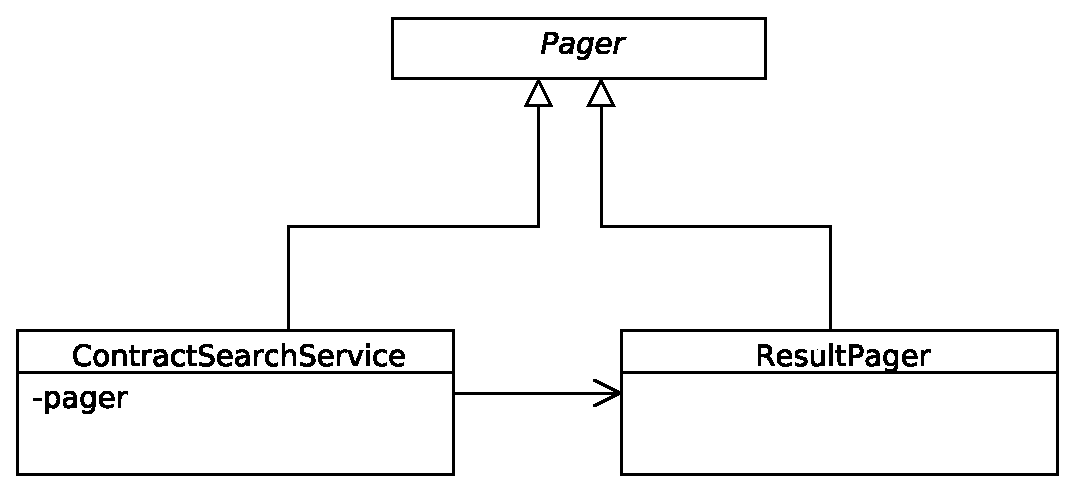
\includegraphics[width=0.7\textwidth]{pager.eps}
\end{figure}

La query è invece costruita utilizzando le Criteria API di JPA, un modo alternativo per costruire query che usa una API Java invece di un linguaggio
come JPQL. Questo tipo di costruzione è specialmente indicata per query dinamiche, ovvero quando non si conoscono i criteri di ricerca fino al runtime.
Il caso che si sta analizzando è proprio quello di una query dinamica: l'utente tramite l'interfaccia messa a disposizione filtra le convenzioni/contributi
in base a vari tipi di criteri.

Volendo usare JPQL si sarebbe dovuto costruire la stringa di definizione della query al runtime, passarla al metodo \lstinline{createQuery} di un
\texttt{Entity Manager} il quale avrebbe parsato la stringa e restituito un oggetto \texttt{Query} da cui sarebbe stato possibile estrarre i risultati.
Ciò significa che ogni volta che si vuole eseguire query è necessario parsare una stringa, costruendo una rappresentazione interna della query per poi generare il codice SQL da
eseguire sul database. Criteria API consente di eliminare l'overhead dovuto al parsing e costruire i vari criteri di ricerca utilizzando una API Java invece
di stringhe. Di seguito è mostrato un estratto di codice usato in \texttt{ContractSearchService} per definire la query.

\begin{lstlisting}

TypedQuery<Contract> query;

CriteriaBuilder cb = em.getCriteriaBuilder();
CriteriaQuery<Contract> c = cb.createQuery(Contract.class);
Root<? extends Contract> agr = c.from(contractClass);

c.select(agr).distinct(true);

List<Predicate> criteria = new ArrayList<Predicate>();

if (companyId != null) {

	ParameterExpression<Integer> p = cb.parameter(Integer.class,
			"companyId");
	criteria.add(cb.equal(agr.get("company").get("id"), p));

}

...


c.where(cb.and(criteria.toArray(new Predicate[0])));
	
query = em.createQuery(c);

if (companyId != null) {
	query.setParameter("companyId", companyId);
	countQuery.setParameter("companyId", companyId);

}

...	

 
\end{lstlisting}

Come si può vedere dall'estratto, per prima cosa si crea una query Root, questa gioca il ruolo di una variabile identificativa in una clausola FROM 
in JPQL e indica a quale tipo di schema si è interessati; quindi con l'operazione \lstinline{select(agr)} si indica quale è il
risultato della query. La clausola WHERE è invece ottenuta componendo una serie di predicati, per esempio con l'espressione
\lstinline{cb.equal(agr.get("company").get("id"), p)} si richiede che l'id della ditta sia uguale ad un certo valore.



